\section{Results}
\subsection{Solution Graph Topology}
The 5-variable SAT instance produced 18 valid solutions forming a connected graph with 80 edges. Structural analysis reveals small-world properties:

\begin{itemize}
    \item \textbf{Diameter}: 3 (maximum shortest path length)
    \item \textbf{Clustering coefficient}: 0.551 (high local connectivity)  
    \item \textbf{Average degree}: 8.89
    \item \textbf{Edge density}: 0.523
\end{itemize}

\begin{figure}[htbp]
\centering
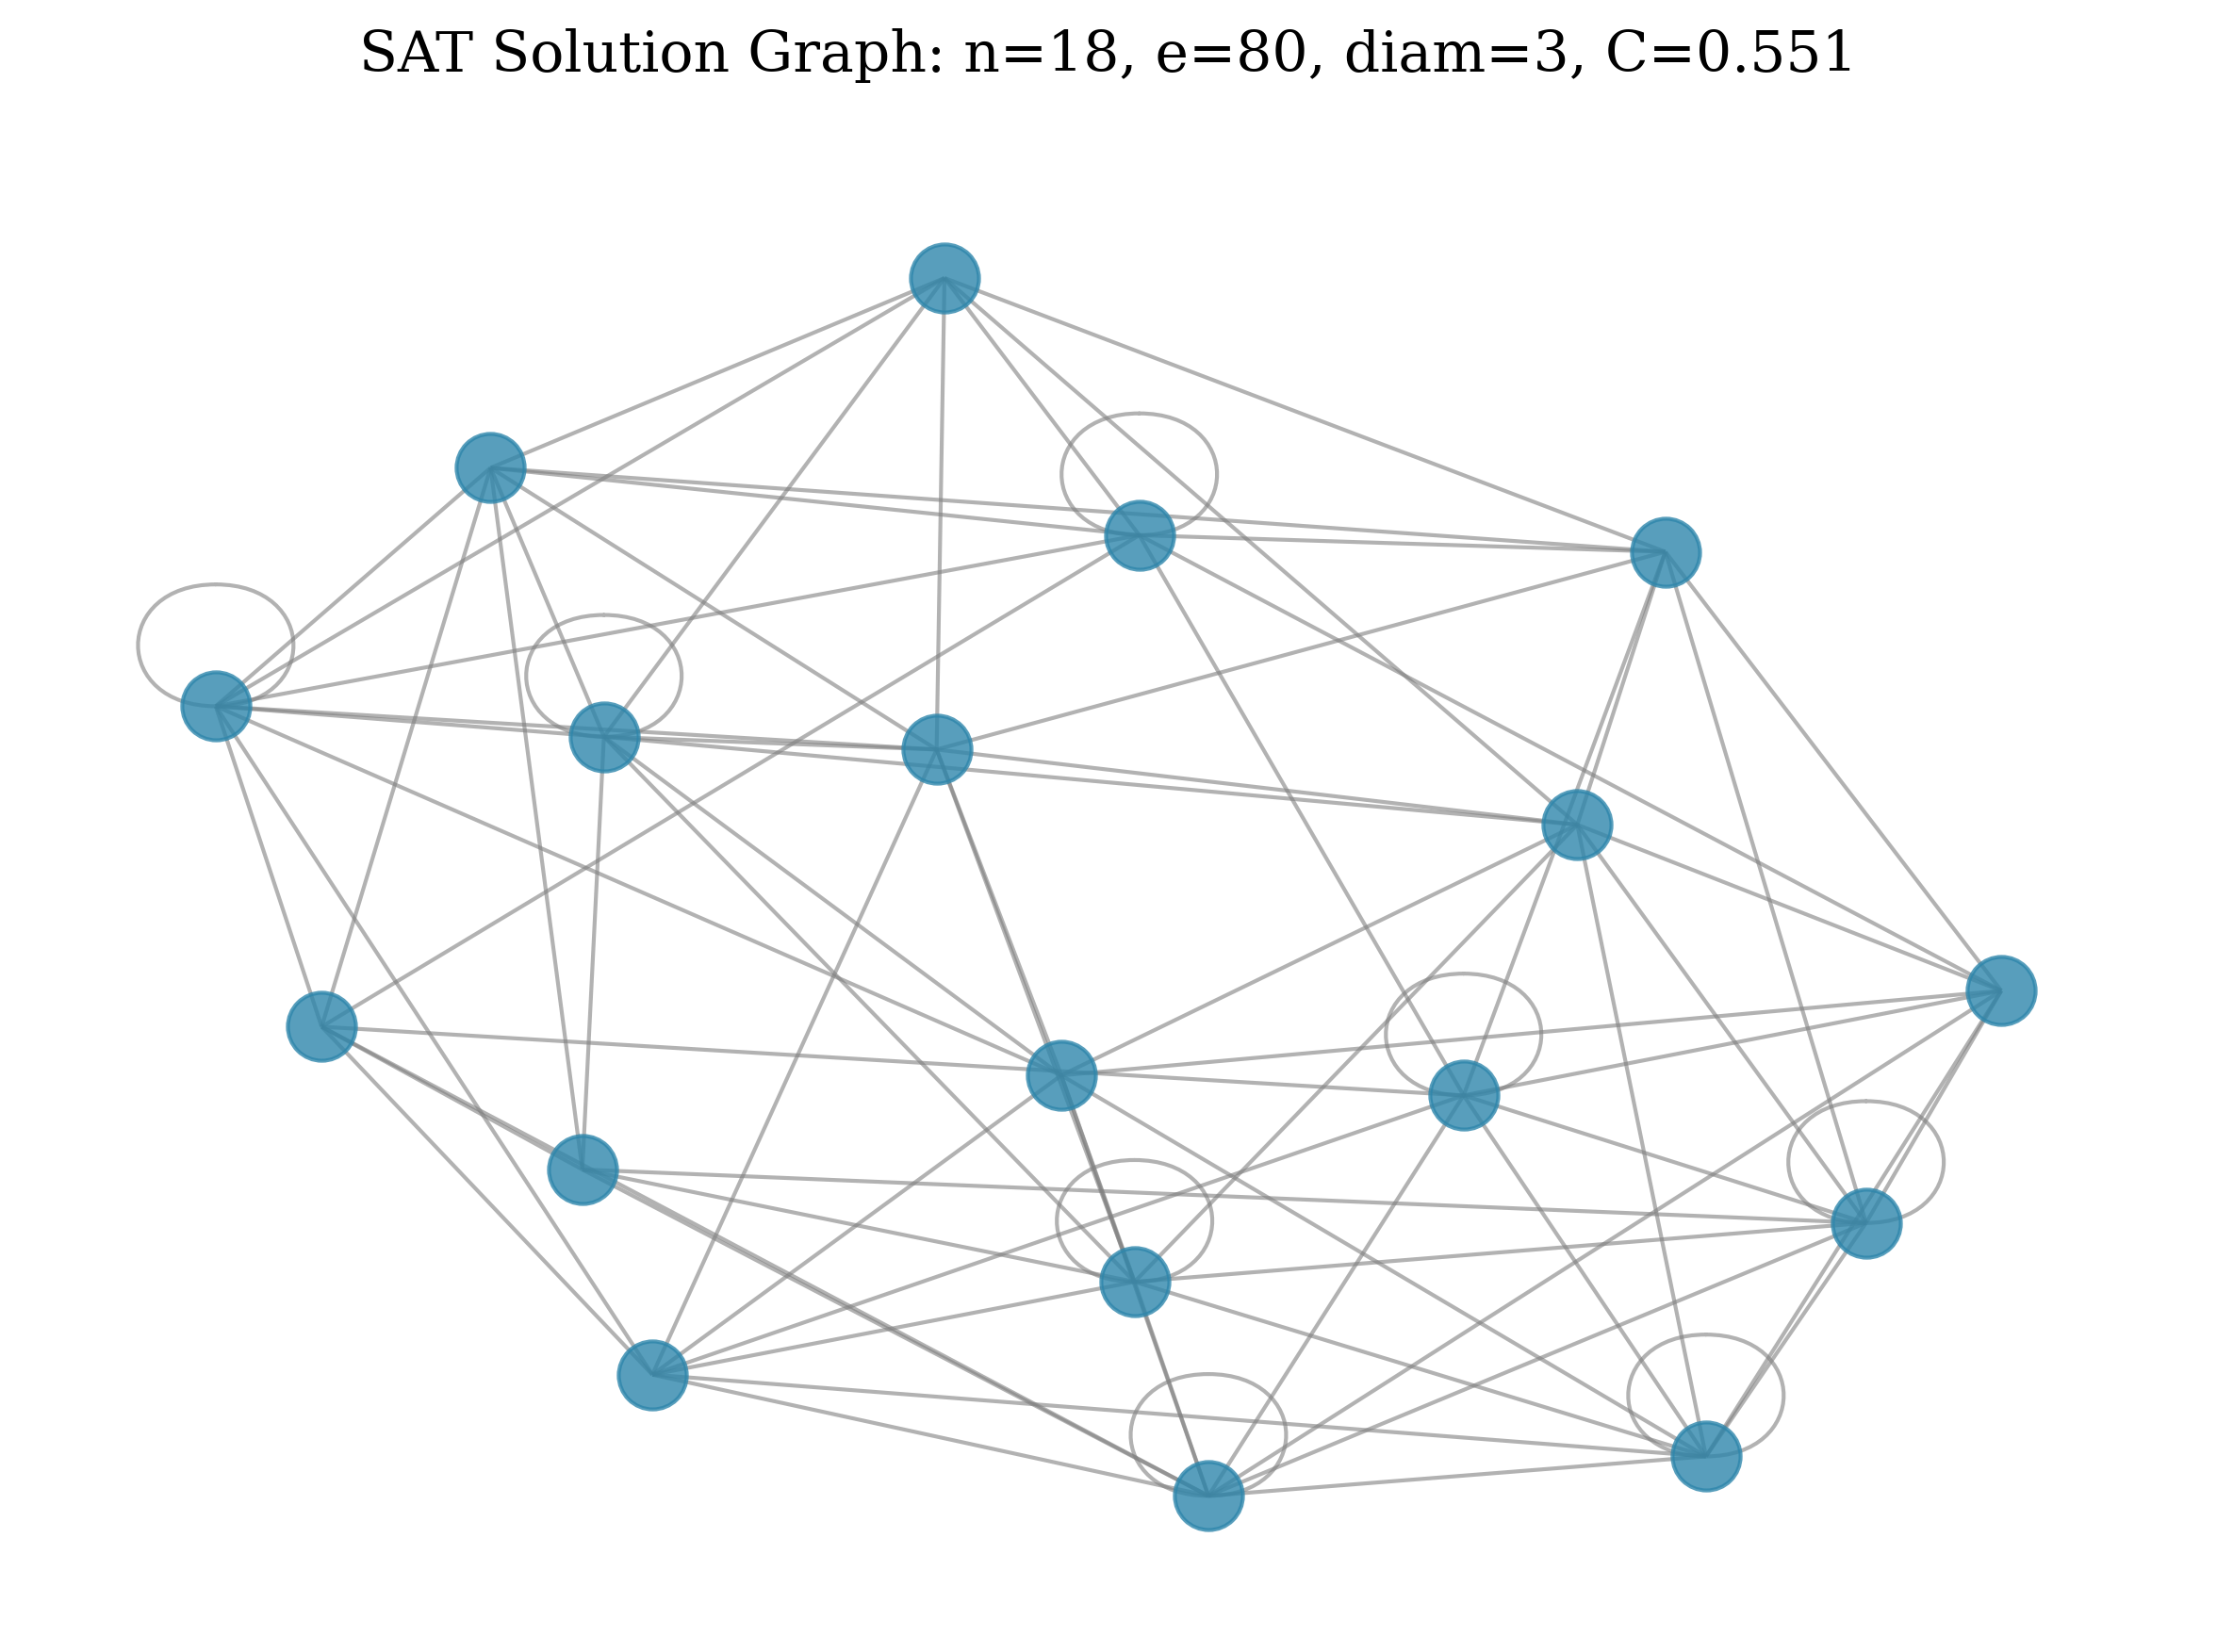
\includegraphics[width=0.9\linewidth]{figures/solution_graph.png}
\caption{Network topology of SAT solution space. The graph exhibits small-world characteristics with high clustering and short path lengths.}
\label{fig:solution_graph}
\end{figure}

\subsection{Quantum Circuit Performance}
The optimized Grover circuit implementation achieved:
\begin{itemize}
    \item \textbf{Qubits}: 5
    \item \textbf{Total gates}: 34
    \item \textbf{Circuit depth}: 10
    \item \textbf{Iterations}: 1 (optimal for $N=32$, $M=18$)
\end{itemize}

Simulation results from 100 shots showed 8 distinct measured states, indicating non-uniform amplitude distribution.
\end{document}
